% Created 2022-06-15 Wed 16:14
% Intended LaTeX compiler: pdflatex
\documentclass[conference]{IEEEtran}
\IEEEoverridecommandlockouts
\usepackage{cite}
\usepackage{amsmath,amssymb,amsfonts}
\usepackage{algorithmic}
\usepackage{graphicx}
\usepackage{textcomp}
\usepackage{xcolor}
\usepackage[hidelinks]{hyperref}
\def \BibTeX{{\rm B\kern-.05em{\sc i\kern-.025em b}\kern-.08em T\kern-.1667em\lower.7ex\hbox{E}\kern-.125emX}}


\author{
  \IEEEauthorblockN{Arnova Abdullah}
  \IEEEauthorblockA{
    \textit{Communication Systems and Networks (Master)} \\
    \textit{Cologne University of Applied Sciences}\\
    Cologne, Germany \\
    arnova.abdullah@smail.th-koeln.de
  }

  \and

  \IEEEauthorblockN{Serkan Kutludag}
  \IEEEauthorblockA{
    \textit{Communication Systems and Networks (Master)} \\
    \textit{Cologne University of Applied Sciences}\\
    Cologne, Germany \\
    serkan.kutludag@smail.th-koeln.de
  }

  \and

  \IEEEauthorblockN{Soumya Sambeet Mohapatra}
  \IEEEauthorblockA{
    \textit{Communication Systems and Networks (Master)} \\
    \textit{Cologne University of Applied Sciences}\\
    Cologne, Germany \\
    soumya\_sambeet.mohapatra@smail.th-koeln.de
  }

  \and

  \IEEEauthorblockN{Adnan Abbas}
  \IEEEauthorblockA{
    \textit{Communication Systems and Networks (Master)} \\
    \textit{Cologne University of Applied Sciences}\\
    Cologne, Germany \\
    adnan.abbas@smail.th-koeln.de
  }
}
  

\date{}
\title{Music Genre Classification using various Machine Learning methods}
\hypersetup{
 pdfauthor={},
 pdftitle={Music Genre Classification using various Machine Learning methods},
 pdfkeywords={},
 pdfsubject={},
 pdfcreator={Emacs 27.2 (Org mode 9.4.4)}, 
 pdflang={English}}
\begin{document}

\maketitle
 \begin{abstract}
Music has been always a part of the human history from the beginning. The music songs differ from each other in terms of style, in other words, genre. Machine Learning can be used for both classification of the genre and to understand the reason behind it. Different machine learning techniques with different preprocessing and some additional implementations are done in this project to see the performance of these models for recognizing music genre. In this paper, the classification models are trained on the Spotify's audio feature dataset. 
 \end{abstract}

 \begin{IEEEkeywords}
machine learning, classification, training, encoding, clustering
 \end{IEEEkeywords}

\section{Introduction}
\label{sec:org59be5e5}

Music is a way of expressing yourself in an abstract way and it has always played a major part in shaping people's emotions. Throughout the ages, different kinds of music have been created, some being very similar and some being distinct. This similarity/distinction is defined as the genre of the music. However, what are the border lines between different genres? Is there any mathematical formulation that gives the correct genre for a given music? Even though the answer is not too obvious, machine learning can be used to learn the relationship between genres. According to the Feng \cite{feng2017music}, Deep Learning with parallell CNN and Bi-RNN works highly effective for music genre classification. In addition, there are lots of different ML models which also give as promising result as DL. In this project, different preprocessing techniques are used to observe their benefits. Different ML models are used to compare and select the best one out of all. Additionally, some extra techniques like hard voting system, semi-supervised learning technique are also used to increase score at the end. All these analysis are implemented with the help of the Scikit-learn \cite{scikit-learn} library.

\section{Setup}
\label{sec:orge536d8d}

\subsection{Data collection}
\label{sec:org54edca5}

The data required for creating the machine learning models was obtained from Spotify. In order to send requests to the Spotify API \cite{spotify} , a spotify developer account was created to obtain a client ID and a client secret. Using these credentials, an authorization token was created. This authorization token was then used to send requests to the "Get Tracks' Audio Features" API end point. A total of 129179 data points consisting of 115 different genres and 19 different features was obtained.

\subsection{Data cleaning}
\label{sec:org49ebdf6}

Upon initial inspection of the dataset, the features \texttt{type}, \texttt{id}, \texttt{uri}, \texttt{track\_href}, \texttt{analysis\_url}, \texttt{year} and \texttt{duration\_ms} were identified to be of no importance as they contain only the meta information about the tracks. Hence these features were removed. Secondly, the dataset consisted of 115 genres. For the purpose of this paper, we reduced the number of target genres to 10. The selected genres were \texttt{acoustic}, \texttt{blues}, \texttt{classical}, \texttt{country}, \texttt{dance}, \texttt{jazz}, \texttt{metal}, \texttt{pop}, \texttt{rock} and \texttt{techno}. The data cleaning process was carried out with the help of the Pandas \cite{reback2020pandas} library in Python.

\subsection{Feature selection and preprocessing}
\label{sec:orgd85df5e}

\begin{figure}[htbp]
\centering
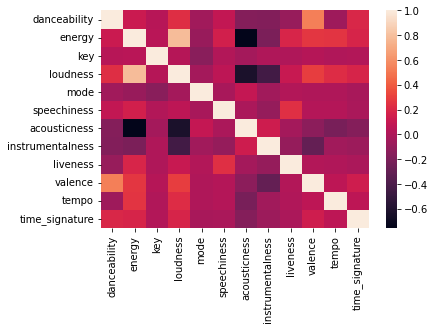
\includegraphics[width=.9\linewidth]{./images/heat_map.png}
\caption{Heatmap of correlation matrix}
\end{figure}

The heatmap of correlation matrix was examined to see the correlation between different features. Based on this, we divided the feature selection and preprocessing into 3 different cases:

\begin{itemize}
\item \textbf{\textbf{Case 1:}} The feature \texttt{key} was removed because it was the least correlated amongst the others. The features \texttt{energy} and \texttt{loudness} were also dropped as they were highly correlated with \texttt{acousticness} as seen from the heatmap of the correlation matrix.

\item \textbf{\textbf{Case 2:}} Since the  genre values are categorical, they were label encoded. Additionally, one-hot encoder was applied for the columns \texttt{mode}, \texttt{key} and \texttt{time\_signature} since these features are categorical in nature.  For the remaining numerical columns, MinMax Scaler was applied. This resulted in the dataset having 27 columns.

\item \textbf{\textbf{Case 3:}} In this case, it was decided to preserve all the features because removing feature decreased accuracy of the machine learning model. Moreover, since our target feature was categorical, the correlation matrix might not have been the correct metric based on which feature selection can be made.
\end{itemize}


\section{Model Training}
\label{sec:org49ca924}

\subsection{Decision Tree Classifier}
\label{sec:org581eced}

A Decision tree \cite{geron2019hands} is a  very versatile machine learning model that make predictions based in a tree like layout. It begins at a root node where it tests whether a condition is satisfied. If the result is true, then it moves to the left child node and if it is false, it moves to the right child node. At the new node, it again tests the condition at that node. This continues until a leaf node is reached and this node gives the final result.

A Decision Tree Classifier was trained preserving all the 12 audio features and the target feature was set to 'genre'. An initial training resulted in a training set accuracy score of 92.3\% and test set accuracy score of 35.8\%. The cross validation accuracy score for 3 folds were 36.6\%, 36.4\% and 35.8\%.

To improve the model, a grid search was used to find the set of hyperparameters that produced the most optimal performance. From the grid search, the best parameter set obtained is as follows:
\begin{itemize}
\item \texttt{max\_depth: 8}
\item \texttt{max\_features: None}
\item \texttt{min\_leaf\_samples: 9}
\item \texttt{min\_samples\_split: 3}
\end{itemize}

Using these hyperparameters, a new Decision Tree classifier was trained. The accuracy scores for the tuned classifier were 47.8\% and 42\% on the training and test set respectively. The cross validation accuracy score improved to 42.5\%.

From these performance metrics, it can be concluded that the Decision Tree Classifier does not perform so well in classifying genres when it is trained with the Spotify dataset.

\subsection{Random Forest Classifier}
\label{sec:org802413d}

Random forest \cite{geron2019hands} is an ensemble supervised machine learning method that works by creating a set of decision trees from a randomly selected subset of the training set. It gives the final prediction by taking majority voting from different decision trees. Random forest is used widely in various applications because it is extremely easy and efficient to train it. Random Forest can reduce the overfitting of data by introducing extra randomness when growing trees.

For traiing the Random Forest Classifier, in addition to the dataset consisting of 10 genres, an additional dataset consisting of 6 genres was also created. The 6 genres were \texttt{acoustic}, \texttt{classical}, \texttt{jazz}, \text{metal}, \texttt{rock}, \texttt{techno}. This was done to compare Random Forest's classification accuracy with reduced number of gernre.

While training this model, the features were encoded as described in \textbf{\textbf{Case 2}}, however none of the features were removed. Stratified train-test splitting was done with 10000 instances in the training set and 2000 instances in the test set. For the additional dataset with 7200 instances and 6 genres, the training set contained 6000 instances, and the test set contained 2000 instances. Applying Random Forest in the dataset with 12000 data points gave an accuracy score of 91.87\% on the training set and 49\% accuracy score on the test set. Similarly, the Random Forest was created with the dataset consisting of 6 genres and it gave 97.87\% accuracy score on the training set and 65.58\% accuracy on the test set.

\begin{figure}[htbp]
\centering
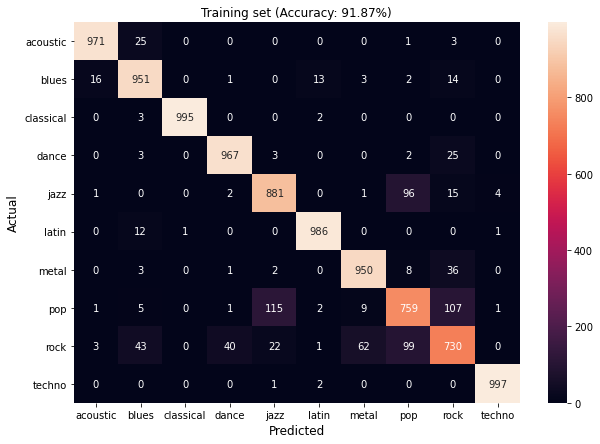
\includegraphics[width=.9\linewidth]{./images/rf_heatmap_train.png}
\caption{Confusion matrix for RF on training data}
\end{figure}

\begin{figure}[htbp]
\centering
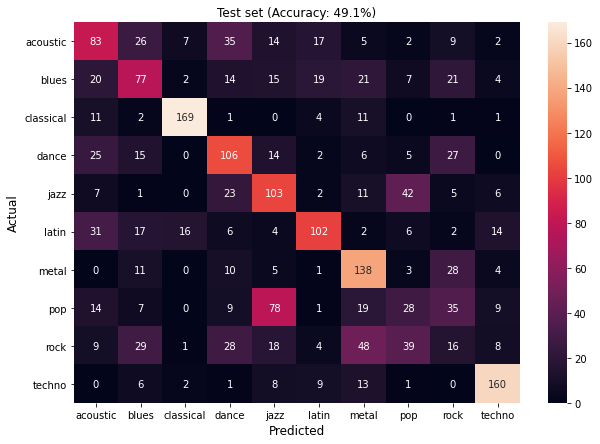
\includegraphics[width=.9\linewidth]{./images/rf_heatmap_test.png}
\caption{Confusion matrix for RF on test data}
\end{figure}

It was observed clearly that RF was overfitting the data. To avoid this, cross-validation and hyperparameter tuning were implemented. The parameters for cross-validation are adjusted, the number of folds is set to 10, allowing shuffling of each class’s sample before splitting and \texttt{random\_state} is set to 42. The adjustable parameters for The RF model are \texttt{n\_estimators}, \texttt{max\_features}, \texttt{max\_depth}, \texttt{min\_samples\_split}, and \texttt{min\_sample\_leaf}. The number of trees in the forest (\texttt{n\_estimator}) is varied between 150, 200, 250, and 300. The maximum depth of the tree (\texttt{max\_depth}) is varied between 20, 26, 32, and 38. The maximum feature (\texttt{max\_feature}) is set to default (\texttt{sqrt}).

From the grid search, the best parameter set obtained for the model trained on dataset with 10 genres is as follows:
\begin{itemize}
\item \texttt{max\_depth: 32}
\item \texttt{max\_features: 'sqrt'}
\item \texttt{min\_leaf\_samples: 7}
\item \texttt{min\_samples\_split: 16}
\item \texttt{n\_estimator: 300}
\end{itemize}

Using these hyperparameters, a new Random Forest classifier was trained. The accuracy scores for the tuned classifier were 49.7\% on the test set. Similar hyperparameter tuning for the model trained on dataset with 6 genres resulted in a test set accuracy score of 65.75\%. Keeping all the features gives approximately 1\% increase in accuracy but it increases computing time in Grid Search. In our case, the computation time is 1556.052 seconds.

Some genres are very similar and so, while predicting those genres, accuracy score gets decreased. In the next section a semi-supervised technique is implemented to identify the best genres for classification.

\subsection{Other models}
\label{sec:org9a42563}

In addition to Decision Tree and Random Forest classifier, several other models were also trained. The models were trained on preprocessed dataset as descirbed in \textbf{\textbf{Case 1}}. 

\begin{itemize}
\item The accuracy of LR on training set was 0.467 whereas on test set is 0.458.
\item The accuracies of KNeighborsClassifier on the training and testing set were 0.429 and 0.414 respectively.
\item For the case of SVM, the accuracy on training and testing were 0.462 and 0.456 respectively.
\item The accuracies of AdaBoostClassifier on training and testing were  0.444 and 0.436 respectively.
\item The accuracies of GradientBoostingClassifier on training and testing were  0.598 and 0.473 respectively.

The best score in this dataset is derived with the hard voting scheme combination of Logistic Regression, Random Forest, GradientBoostClassifier and SVM. This gave an accuracy of 0.552 on the training set and 0.480 on the test set.
\end{itemize}



\section{Semi-supervised approach}
\label{sec:orgb8f7151}

After training and evaluating several models, we found that the accuracy was still low. One of the main reasons for this was that the genres that was selected initially were having very strong similarities amongst each other. The genres were selected by intuition based on their current popularity. However, technically some genre were very difficult to distinguish by the machine learning models. For example, the audio features of the genre rock have strong similarities with that of pop, techno has strong similarity to metal and classical is very close to country. In order to improve the classification accuracy, we therefore needed to select a set of genres that are very distinct.

In the final attempt, we took a semi-supervised learning approach to identify genres that are distinct from each other. Our initial idea was to identify clusters of similar genres using the KMeans \cite{geron2019hands} method. But this method failed to recognize any clusters due to the nature of the Spotify dataset. Therefore, we we manually defined grid of clusters and selected the genre that has highest count in that grid.

For our purpose of creating distinct cluster regions, we required comparison of two features that have the data points spread through out the X-Y plane so that every grid would contain uniform number of data points. From the scatter matrix of the dataset, the comparison between the features \texttt{acousticness} and \texttt{valence} were chosen to be the best candidate for creating grids. The two features were segmented into 9 different grids and the genre having the highest count in each grid was identified.

\begin{figure}[htbp]
\centering
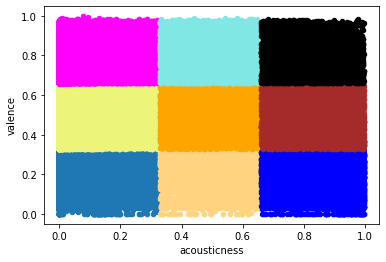
\includegraphics[width=.9\linewidth]{./images/grid_cluster.png}
\caption{Manually defined Grid cluster}
\end{figure}

 From the grids, the following genres were identified to have maximum count: \texttt{black-metal}, \texttt{mandopop},
\texttt{classical}, \texttt{grunge}, \texttt{sertanejo}, \texttt{tango}, \texttt{reggae}, \texttt{salsa}, \texttt{tango}. The rows containing these genres were extracted from the original dataset. The new dataset contained 9200 instances. A train-test split was created with 20\% ratio and the training set was used to retrain a Random Forest classifier.

With the new model, an accuracy score of 99.99\% was obtained on the training set and 80.70\% on the test set. The 3 fold cross validation scores obtained were 81.37\%, 79.9, 81.08\%.

From the performance metrics obtained with the new list of genres, it can be concluded that if the genres are distinct enough, the model is capable to classify new data with much higher accuracy.

\section{Results}
\label{sec:org68c7fdd}

\begin{table}[htbp]
\caption{Accuracies of various models}
\begin{center}
\begin{tabular}{|c|c|c|}
\hline
\textbf{Training Models} & \textbf{Training set accuracy} & \textbf{Test set accuracy} \\
\hline
Decision Tree & 47.84\% & 42.08\% \\
\hline 
Random Forest & 64.9\% & 49.7\% \\
\hline
Logistic Regression & 46.7\% & 45.8\% \\
\hline
KNC & 42.9\% & 41.4\% \\
\hline
SVM & 46.2\% & 45.2\% \\
\hline
ADA & 44.4\% & 43.6\% \\
\hline
GBC & 59.8\% & 47.3\% \\
\hline                             
\end{tabular}
\end{center}
\end{table}

\begin{figure}[htbp]
\centering
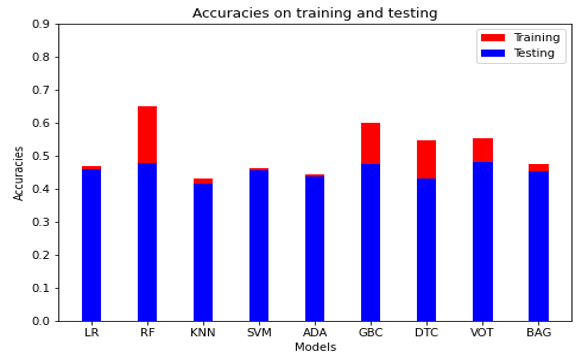
\includegraphics[width=.9\linewidth]{./images/model_comparison.png}
\caption{Accuracies of various models}
\end{figure}

\section{Conclusions}
\label{sec:org59ccc4b}

In this paper, various machine learning methods to classify genre of music were discussed. From the results, it can be concluded that the Random Forest model is the most suitable model for this purpose. It was also seen that the selection of target genres affected the accuracy of the model. Therefore, for higher accuracy, it is necessary to select the genres which are very distinct and different from each other.


\bibliographystyle{unsrt}
\bibliography{references}
\end{document}
